%%%%%%%%%%%%%%%%%%%%%%%%%%%%%%%%%%%%%%%%%%%%%%%%%%%%%%%
%%                   Introduction                    %%
%%%%%%%%%%%%%%%%%%%%%%%%%%%%%%%%%%%%%%%%%%%%%%%%%%%%%%%
\chapter{Introduction}
\chaptermark{Introduction}
\label{ch:intro}
%%%%%%%%%%%%%%%%%%%%%%%%%%%%%%%%%%%%%%%%%%%%%%%%%%%%%%%

The development of aerospace systems relies on the definition and communication of design requirements from the stakeholders to the \acp{OEM}, who then define and communicate design requirements to the suppliers of components. In this context, design requirements specify for each manufacturing organization what the components shall achieve in order to provide value to stakeholders once integrated as part of a system \cite{Blanchard1981}. While requirements are supposed to be clear and well-defined, they are subject to changes during a development project \cite{Peterson2007}. Due to the large number of stakeholders and design teams involved in the design of complex products, requirements are in constant flux even after a product has been commissioned. 

We consider the aerospace industry as an example. Requirement changes occur for a plethora of reasons \cite{Boeing2013,Eckert2004}. The temperature loads a structural component must sustain in operation may change during product development due to a shift in the engine architecture specified by the engine \ac{OEM}. Furthermore, requirements may change during the in-service phase due to changes in the market or in the legislation that governs the industry. There is an inherent uncertainty in design requirements at the beginning of a product development project, which gradually decreases as the project advances and decisions are made. At the beginning, where the innovation potential is high, such uncertainty can be very large \cite{ullman2009mechanical}. In the early phases, design requirements are normally communicated as ranges, and the final requirement (e.g. temperature load) may lie anywhere in this range (or in some cases, even outside).

If the product's specifications fall short of the requirements during development or product lifecycle, an upgrade to the specifications is warranted to maintain functionality. This may involve a complete redesign of the product depending on the severity of the required changes. Complete redesign involves discarding the current iteration of the product and starting a new development cycle with the changed requirements as inputs. This cradle-to-grave approach is extremely inefficient when considering a \ac{CE} where value is generated from each unit of resource by recovering and regenerating products and materials at the end of each service life \cite{MacArthur2013b}. In order to increase the recoverability of the product, and avoid loss in value due to disposal, products should be designed for such activities in order to increase their relevance in a \ac{CE} and extract as much value from them as possible. Recovering a product involves returning its specifications to its pre-disposal levels. However, requirements are seldom the same after a product's lifecycle has run its course. As a result, the product's specifications have to be upgraded to meet the set of requirements expected of current generation products. Designing products for such unforeseeable requirements is the main subject of this thesis.

This thesis utilizes numerical methods for addressing the problem of designing prod\-ucts for remanufacturing activities where requirements are expected to be highly dynamic. In this chapter, Section \ref{sec:motivation} provides motivation for implementing the design para\-digms introduced in this thesis to mitigate the challenges that arise due to changing product requirements. The research objectives of this thesis are then discussed in the context of product remanufacturing design problems. The contributions of this thesis to the field of engineering design for uncertain requirements are then outlined in Section~\ref{sec:contribution}. The chapter concludes by outlining the remainder of the thesis in Section \ref{sec:outline}.

%============================= MOTIVATION ==============================%
\section{Motivation}
\label{sec:motivation}

The increasing environmental impact of industrial activities is changing the perception of legislators and business enterprises towards the importance of recovering value from products that have reached the end of their useful lifecycles, especially if this end is brought about by an unforeseen change in requirements or specifications. As a result, a new paradigm for product design has become increasingly relevant in modern economies.

%---------------------------------------------------------------------%
% Circular economy
\subsection{Circular economy and product recovery} \label{subsec:CE}

A \ac{CE} can be used to return products that have reached the end of their useful lifecycles into service and extract as much value from them as possible. \ac{CE} helps achieve both economic growth and environmental protection. Since resources are limited, legislation has been put forth so that business enterprises bear responsibility for the environmental, social and economic impacts their products have on society \cite{Matos2007}. This caused business enterprises to adopt sustainable development practices when designing their products.

A \ac{CLSC} can return used or discarded products to working condition. This enables sustainable development by reducing the environmental impact of products \cite{QuariguasiFrotaNeto2010}. A \ac{CLSC} includes a forward supply chain where products are used normally until the end of their life and a reverse supply chain that returns the discarded products to a previous stage in its lifecycle. Examples of recovery activities in a reverse supply chain include remanufacturing, reuse and recycling \cite{Lieder2016,MacArthur2013a}. Since \ac{CE} encompasses products as well as their forward and reverse supply chains, businesses must design their products for closed-loop product recovery activities \cite{Lieder2016}. This includes design for remanufacturing, recycling and reuse. In this thesis, we focus on remanufacturing since it is more sustainable than recycling and recovers more value across the supply chain due to increased virgin material substitution and retention of the embodied energy used to manufacture the original product from the raw materials \cite{MacArthur2013a,Goodall2014}. 

There is a number of studies that consider product design for remanufacturing \cite{Ijomah2010,Liu2017}. However, the majority focus on closed-loop supply chain logistics of remanufacturing \cite{Mahadevan,Golinska2015,VanThao2015,Song2005,Koren2018}. Product remanufacturing design problems are more challenging to address due to the variable design requirements encountered during product design. Studies that focus on remanufacturing design are reviewed in Section \ref{sec:remanufacturingdesign}. 

Design for remanufacturing rules found in the literature specify that a product's components should allow room for modifications to meet design requirements \cite{Ijomah2009}. Furthermore, it is important to distinguish refurbishment from remanufacturing: the former is used to satisfy original specifications, whereas the latter allows for considering changed requirements. As a result, products should be designed for changing requirements to enable product recovery by remanufacturing.

%---------------------------------------------------------------------%
% Design for changing requirements
\subsection{Designing for changing requirements} \label{subsec:changingreq}

Design requirements are subject to change during a product's lifecycle \cite{Goodall2014,Lindahl2007,Thierry2012,American2017}. Variable parameters such as customer requirements and loading conditions influence des\-ign requirements such as cost and product life requirements \cite{Fricke2005} and can be unpredictable despite the best efforts of forecasters and analysts \cite{DeNeufville2011}.

Design \textit{changeability} enables designs to change through a number of change mechanisms whose aspects can include flexibility, agility, robustness, and adaptability. A number of basic and extended principles have been identified as enablers of design changeability \cite{Fricke2005}. In this thesis we focus on two aspects of changeability, flexibility and robustness in product design for accommodating uncertain requirements. Advances in incorporating design changeability in product design are reviewed in Section~\ref{sec:changeability}.

The first contribution of this thesis provides a rigorous formulation for flexibility in terms of \textit{scalability}. Scalability is an aspect of flexibility which is defined in the literature and expanded upon in Section \ref{sec:changeability}. Scalability is highly relevant to remanufacturing design problems as will be explained in Chapter~\ref{ch:background}. Decisions regarding the scalability of a remanufacturing design are made based on current information that is available to the designer. The issue of designing a product based on the current state of the product and its corresponding requirements has been addressed by \citeauthor{Alhandawi2020} \cite{Alhandawi2020}.

However, requirements change over the course of a product development project or life\-cycle. A decision-making tool based on past and current information is required \cite{Eckert2019}. The second contribution of this thesis formulates and quantifies design flexibility and robustness over the course of a remanufacturing design process. Decisions about the desired amount of flexibility and robustness are made based on current and past information from the design process or the product lifecycle.

The motivation for such a decision-making tool stems from conventional design practices with regards to changing requirements. We use a thought experiment to provide motivation for the research presented in this thesis.

%---------------------------------------------------------------------%
% Motivation problem
\subsection{A thought experiment} \label{subsec:thoughtexperiment}

Designers address changing requirements using different design strategies. One strat\-egy involves frequent redesign of the component as system requirements are constantly updated and cascaded down to the component level \cite{Eckert2004}. This is an example of \textit{flexible} design. Another strategy for managing change is by building design \textit{margins} into the component such that it incorporates a buffer against change \cite{Clarkson2004,Eckert2004}. Several researchers have developed metrics for these quantities which are reviewed in Section~\ref{sec:margins}. This buffer helps reduce the amount of redesign needed to satisfy an uncertain set of requirements by \textit{absorbing} change. This is an example of a \textit{robust} design. Flexibility and robustness are two ends of a spectrum in terms of design changeability and balance between the two can help mitigate unnecessary overdesign. Let us consider a problem from the industry and explore our options for tackling it.

\begin{figure}[h!]
	\centering
	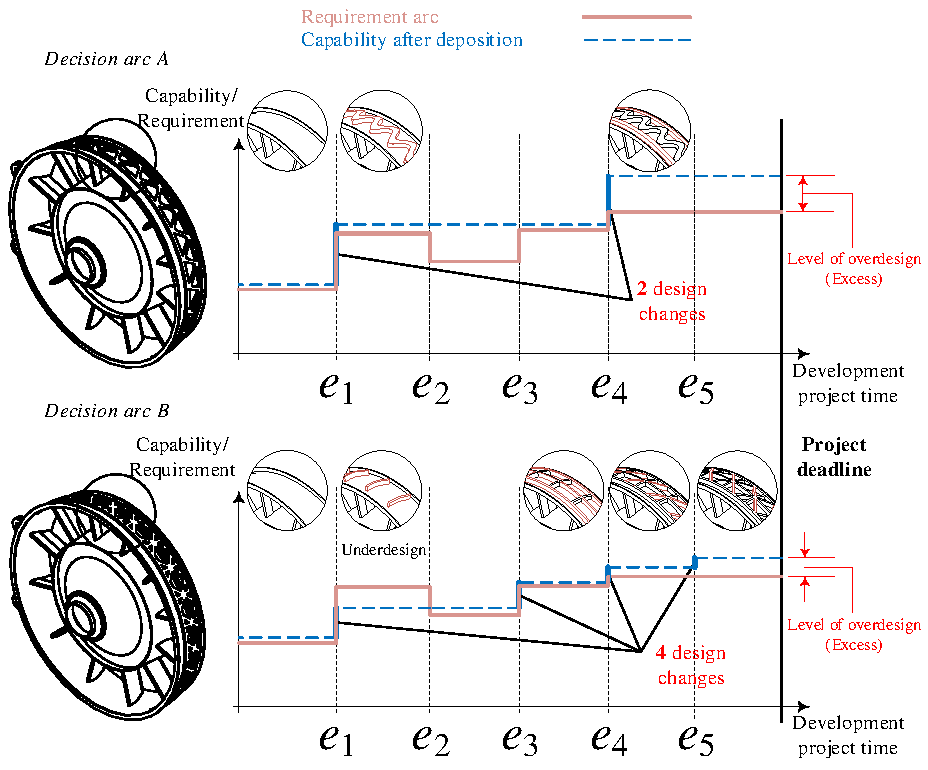
\includegraphics[width=0.9\textwidth]{problem_description.pdf}
	\caption{Example product development project showcasing different decision arcs}
	\label{fig:problemdescription}
\end{figure}

A \acf{TRS} (a static structural component in an aeroengine) must sustain temperature loads as a result of the hot engine exhaust gases. These temperature loads can change during the course of a development project or during the in-service phases. In Figure~\ref{fig:problemdescription}, these changes are represented by the “requirement arc” (red line). For simplicity, in this example the temperature requirement is assumed to change five times, in conjunction with critical design reviews \cite{Cooper2008}. The period of time in which a requirement is held constant is referred to as an \textit{epoch} \cite{McManus2007}. The benefit of using \ac{AM} for remanufacturing the \ac{TRS} is exemplified by two decision \textit{arc}s A and B. The terms epoch and arc are expanded upon in Chapter~\ref{ch:TSEcont}. With \ac{AM}, the geometry of the \ac{TRS} can be initially designed ($e_1$) to meet the lower bound of the temperature range, while depositing a stiffener on the structure as the temperature requirement changes. This strategy resonates well with flexible design principles, which suggest designing for a relatively low capability that can be expanded if changes occur \cite{DeNeufville2011}. However, the decisions made during the design of the stiffener’s geometry may impact such flexibility substantially. For instance, choosing the deposit geometry given by decision arc A at $e_2$ (wavy design concept) will result in a design with a capacity that fulfils the new requirement. However, further changes of this geometry (such as the one made at $e_4$) do not allow for close tracking of the requirement arc, resulting in overdesign (the blue line in Figure~\ref{fig:problemdescription}). On the other hand, decision arc B (hatched design concept) allows for a better tracking of the requirement arc. This reduces the risk for overdesign at the end of the project. However, this comes with the cost and effort of performing more depositions during the course of the development (4 instead of 2) which are costly and time consuming, outweighing the benefits given by this more flexible decision arc. Furthermore, the capability is lower than the requirement in some cases which may not always be acceptable during a development project.

This example draws inspiration from the contrast in longevity of the B-52 stratofortress bomber and F/A-18 hornet. The B-52 enjoyed a longer service cycle and was able to cope with the needed modifications due to technological advancements as opposed to the F/A-18 hornet. This was due to the embedded design margins (in the form of excess) during initial production of the B-52. The F/A-18 hornet had more \textit{modularity} (a form of flexibility) to counteract the reduced margins available for upgrade but still suffered greatly once the margins were consumed during its service life requiring a complete redesign \cite{Long2017}. This case study underscores the necessity for quantifying and strategically allocating design margins in product design.

We aim to address the shortcomings of either design strategy that were identified in this thought experiment. We formulate the thesis objectives accordingly.

%---------------------------------------------------------------------%
% Thesis objectives
\subsection{Objectives} \label{subsec:objectives}

% Furthermore, there is a trade-off between the flexibility that can be enabled by \ac{AM} and other attributes of the design (such as weight, manufacturing costs and excess) that need to be optimized in the early design phases. We review a number of studies that utilize tradespace exploration strategies so that the tradeoff between product costs and its degree of flexibility or robustness as given by the metrics developed in this thesis can be studied. These studies are summarized in Section~\ref{sec:tradespace}.

% Arguably, a set of changeable solutions is required to leverage the added design changeability in order to provide possible alternative designs. \Acf{SBD} is a design paradigm that places emphasis on a varied solution set as a means for accommodating uncertain requirements. Consequently, results from both contributions of this thesis are presented as sets of design solutions by employing the principles of \ac{SBD}. Feasibility of the solutions with respect to the requirements and changeability must be checked and maintained throughout the solution set. Advances in \ac{SBD} are reviewed in Section~\ref{sec:SBD}.

% Having explained the rationale behind the scope and motivation of this thesis, we outline the objectives and contributions in the following section.

The goal of this thesis is to develop several design frameworks for managing uncertain design requirements during the product development process or throughout its lifecycle. 

The frameworks developed in this thesis follow the principles of \acf{SBD} by providing a set of feasible design solutions in order to leverage the added design changeability from our frameworks. 

Feasibility is assessed using engineering models which can be computationally intensive. Specifically, remanufacturing design problems involving \ac{AM} feature thermomechanical models with coupled thermal and structural analyses of the deposition process. These thermomechanical models are developed for the \ac{TRS} described earlier as it will be used as a remanufacturing design problem to demonstrate our methods. The thermomechanical models are evaluated prior to assessing the feasibility of the design in terms of its structural performance. In order to navigate the design space with relative ease in search of the solution sets respective of each framework, a surrogate model is obtained by training a response surface model with data obtained from the thermomechanical/engineering model.

Decisions are rendered in each framework using rigorous derivative-free optimization algorithms. This is due to the non-smooth response that can be exhibited by the thermomechanical/engineering models and their surrogates.

The first framework provides decisions about the design variables in order to maintain scalability in the set of design solutions given current information about the state of the design problem. Parametric design optimization is used to assess feasibility while maximizing structural performance to obtain a set of parametric optimal designs in the design space. A response surface of the optimization solutions with respect to the parameters governing the design requirements is constructed in the parameters space. A scalability constraint based on the manufacturing process used is formulated in the parameters space and used to identify scalable design solutions that can be mapped back to the design space.

The second design framework provides decisions regarding design variables such that overdesign (excess) is minimized throughout the different stages of the development process or the product lifecycle while maintaining a threshold reliability level with respect to uncertain requirements. Monte Carlo integration is used at each stage where decisions are made to quantify the reliability (probability of satisfying a requirement governed by a joint probability density function) and excess. Additionally, metrics for quantifying flexibility and robustness are developed as part of this framework. Monte Carlo simulation is used to generate and chain together different requirements. Corresponding design decisions are obtained by solving a combinatorial optimization problem. This results in sets of optimal, flexible, and robust design solutions. The effect of minimizing excess on robustness and flexibility is investigated via tradespace exploration.

The objectives are summarized as follows.

\begin{itemize}
	\item{Develop a framework for identifying design solutions that have the greatest potential for remanufacturing.}
	\item{Strategically quantify and allocate the aspects of design flexibility and robustness to address changing requirements during remanufacturing.}
	\item{Provide a sufficiently diverse set of equally reamnufacturable solutions to provide designers with alternatives after committing to a particular solution.}
\end{itemize}

% \begin{itemize}
% 	\item{Utilize the principles of \ac{SBD} to obtain sets of design solutions}
% 	\item{Utilize rigorous derivative-free optimization algorithms since we use engineering models that are prone to nonsmooth responses}
% 	\item{Use parametric design optimization to obtain a set of feasible design solutions for an instance during the product development process or during its lifecycle}
% 	\item{Use response surface of parametric optimization solutions to map between design and parameters spaces}
% 	\item{Formulate and use a scalability constraint in the parameters space to identify scalable optimal designs}
% 	\item{Compute instantaneous reliability and excess for a particular design and requirement at a certain stage in its product development process or lifecycle}
% 	\item {Minimize cumulative excess throughout product development process or lifecycle to mitigate overdesign}
% 	\item{Obtain sets of optimal, flexible and robust design solutions corresponding to different product development or lifecycle scenarios}
% \end{itemize}
%=========================== CONTRIBUTIONS =============================%
%============================= MOTIVATION ==============================%
\section{Contributions}
\label{sec:contribution}

The contributions of this thesis are as follows.

\begin{enumerate}
	\item{An \ac{SBD} framework for identifying sets of parametric optimal designs and scalable optimal designs.}
	
	The following metrics and algorithms were developed as part of this framework.
	
	\begin{enumerate}
		\item{A surrogate enabled parametric optimization scheme using derivative free methods for obtaining parametric optimal designs.}
		\item{A response surface methodology for performing post optimality analysis on the parametric optimal designs and evaluating their scalability.}
		\item{A scalability constraint formulated in the parameters space}
		\item{A methodology for mapping scalable optimal designs from the parameters space to the design space using random sampling techniques.}
	\end{enumerate}
	%
	\item{A design margin quantification and allocation tool for addressing changing requirements throughout a product's lifecycle or development process.}
	
	The following metrics and algorithms were developed as part of this framework.
	
	\begin{enumerate}
		\item{A method for computing reliability and excess of a particular design and requirement using Monte Carlo integration.}
		\item{A method for generating different product development or lifecycle scenarios using Monte Carlo simulation and importance sampling.}
		\item{An \ac{SBD} combinatorial optimization approach for obtaining sets of optimal designs.}
		\item{An \ac{SBD} method for obtaining flexible and robust sets of solutions.}
		\item{A tradespace exploration strategy for visualizing and comparing flexible, robust and optimal sets of solutions.}
	\end{enumerate}
\end{enumerate}

The contributions of this thesis have been tested and applied to the following industrial case studies.

\begin{enumerate}
	\item{Parametric optimal and scalable \ac{SBD} solutions were obtained for a \ac{TRS} remanufacturing problem involving deposition of a simple circumferential stiffener subject to internal pressure loads.}
	\item{Sets of optimal, robust and flexible design sequences were obtained for a problem involving the deposition of a stiffener on the outer casing of a \ac{TRS} subject to multiple uncertain temperature loads.}
\end{enumerate}

%============================== OUTLINE ================================%
\section{Outline}
\label{sec:outline}

The thesis is organized through the following chapters. Chapter \ref{ch:background} presents a detailed literature review of the main aspects featured in our contributions. We review literature related to remanufacturing design, design changeability, design margins, \ac{SBD}, and tradespace exploration. Chapter \ref{ch:thermomechanical} presents the thermomechanical models used to model the \ac{AM} remanufacturing process of a \ac{TRS} used in both frameworks as described in subsequent chapters. Chapter \ref{ch:scalableSBD} describes a \ac{SBD} framework for identifying scalable optimal designs during an instant in the product development process or lifecycle. An application problem based on the remanufacturing of a \ac{TRS} subject to varying requirements and loads is used to demonstrate the framework. Chapter \ref{ch:TSEcont} presents a framework for minimizing design excess throughout the product development process or lifecycle while maintaining a threshold reliability given uncertain requirements. The \ac{TRS} remanufacturing problem used for demonstrating this framework is modified to feature multiple distinct stages at which design decisions must be made. \ac{SBD} results are obtained using the described framework for minimizing excess and are compared against flexible and robust design sets using tradespace exploration. Chapter \ref{ch:stohasticopt} discusses the application of stochastic optimization algorithms for providing sets of design solutions when requirements are uncertain. Based on the results of stochastic optimization, recommendations for improving the frameworks in Chapters \ref{ch:scalableSBD} and \ref{ch:TSEcont} are made. The conclusion and thesis contributions are presented in Chapter \ref{ch:conclusion}.